% %This is a very basic essay template based on letter class.
\documentclass[12pt,a4paper]{article}
\usepackage{ucs}
\usepackage[T2A]{fontenc} 
\usepackage[utf8]{inputenc}
\usepackage[english,bulgarian]{babel} 
\usepackage[margin=1in]{geometry}
% \usepackage[bindingoffset=2cm,centering,includeheadfoot,margin=1in]{geometry}
\usepackage{graphicx}
\usepackage{setspace}
\onehalfspacing


\begin{document}

\thispagestyle{empty}
\begin{titlepage}
\begin{center}
\newcommand{\HRule}{\rule{\linewidth}{0.5mm}}

% Upper part of the page
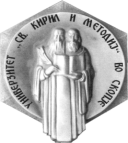
\includegraphics[width=0.15\textwidth]{images/ukim}\\[1cm]
\textsc{\large Универзитет „Св. Кирил и Методиј“ - Скопје}\\[1.5cm]


\includegraphics[width=0.3\textwidth]{images/finki_logo}\\[1cm]
\textsc{\large Факултет за информатички науки и компјутерско
инженерство}\\[1.5cm]

% Title
\HRule \\[0.4cm]
{  \bfseries \textsc{Преземање сознанија без наведување на изворот (плагијат)} \\[0.4cm] - есеј
-}
\\[0.4cm]

\HRule \\[1.5cm]

% Author and supervisor
\begin{minipage}{0.45\textwidth}
\begin{flushleft} 
\emph{Студент:}\\
М-р Томче \textsc{Делев}\\
tomche.delev@finki.ukim.mk
\end{flushleft}
\end{minipage}
\begin{minipage}{0.45\textwidth}
\begin{flushright} 
\emph{Ментор:} \\
Д-р Кирил \textsc{Темков}
\end{flushright}
\end{minipage}

\vfill

% Bottom of the page
{\large Јуни 2012}

\end{center}
\end{titlepage}

Според Merriam-Webster Online Dictionary, „плагијаризам“ е: 
\begin{itemize}
  \renewcommand\labelitemi{--}
  \item да се украдат и да се користат идеите или зборовите на други автори како
  свои
  \item да се искористи туѓо достигање без да се наведе изворот
  \item буквално да се украде
  \item да се претстави како нова и оригинална идеја или продукт кој произлегува
  од постоечки извор.\footnote{Превод од англиски: авторот}
\end{itemize}

Неодамна во јавноста беа обелоденети два случаи на плагијатори. Во првиот случај
на германскиот Министер за одбрана, Карл-Теодор цу Гутенберг (Karl-Theodor zu
Guttenberg) му беше одземена докторската титула за неговиот труд предаден на
Универзитетот во Бејрут, што резултираше и со неговата прерана оставка од
министерската позиција во владата на Канцеларката Ангела Меркел. Неговата
харизма како политичар и неговото аристократско потекло, пред скандалот со
плагијаризам, го ставаа на врвот од листата на луѓе кои можеби ќе ја наследат
сегашната германска канцеларка. Во моментот тој е само бледо сеќавање и покрај
тоа што тој е првиот министер за одбрана кој по Втората светска војна има
постигнато многу значителни реформи во одбранбената политика на Германија.

Во вториот случај, Претседателот на Унгарија, Пал Шмит, беше принуден да си даде
оставка. Повикувајќи се на унгарскиот устав, Претседателот на државата треба да
го обединува народот, а во моментот кога неговиот личен проблем почнал да го
разделува народот тој сметал дека треба да престане да ја врши својата должност
и да го предаде својот претседателски мандат. Оставката следи не долго откако
Универзитетот во Будимпешта му ја одзема докторската титула доделена во 1992
година, поради како што тој самиот изјавува „неосновани обвинувања“ за нелегално
и неморално користење на туѓи достигања без наведување на изворот. Овие два
случаи стануваат актуални во последните две години и ја разбрануваа светската
јавност. Како академски граѓани кои се придржуваат кон истите морални и етички
вредности и кои налагаат заштита на интелектуалната сопственост, актот на
плагијаризам е сериозно прекршување на истите, без оглед на тоа дали станува
збор за намерно или ненамерно користење на туѓи достигања.

Проблемот ``copy-paste'' како што е познат во пошироката јавност станува сѐ
посериозен во последните години. Постојаниот напредок на информатичката
технологија, доведува до зголемената достапност на научни извори и достигања на
интернет. Нивното пресликување на неколку веб страни без додржување на
соодветен систем на цитати и нивното последователно користење како кредибилни
извори во работата, претставува сериозна опасност во работата на младите и
неискусни истражувачи.
 
Плагијаризмот, самиот по себе, не само што претставува кривично дело за кое што
обвинетите одговараат пред суд, туку автоматски го уништува академскиот углед и 
кредибилитет на научникот. Штом истиот ќе биде докажан, се преиспитуваат сите
поранешни достигнувања на истиот научник. Моменталната дебата за тоа дали
интернетот го повредува/злоупотребува правото на интелектуална сопственост може
слободно да биде пренесена и во академската средина. Истите тие научници кои
наместо да истражуваат го поминуваат времето барајќи зборови, реченици,
апликации и продукти кои може да си ги земат за свои, ги осудува и Универзитетот
„Св. Кирил и Методиј“. Во својот Етички кодекс експлицитно во одделот 4
„Етичките вредности во односите на Универзитетот“ параграф 5 и одделот 5 „Етика
во науката и во високото образование“ параграф 5 наведува дека УКИМ
„посебни напори вложува против нелегалното и неморално користење на туѓи
достигања (плагијат)“ и дека „не се манипулира со научните сознанија, ниту се
користат за нехумани и неетички цели“. Понатаму тврди дека доколку се докажат
вакви постапки истите ќе бидат санкционирани, а меѓу нив плагијатот ќе биде
најстрого осуден. Со тоа УКИМ застанува на страната на авторите и го штити
нивното право на интелектуална сопственост.\footnote{Етички Кодекс на УКИМ во Скопје.}

Интересен аспект од оваа дебата е токму оној кој произлегува од информационата
револуција. Во време кога сите податоци и извори стануваат сѐ подостапни и
нивната употреба подлежи на сѐ поголема злоупотреба, нашата обврска како
компјутерски и информатички инженери е да постапуваме етички и совесно со
информациите кои ни се потребни и кои ги поседуваме за да можеме да твориме
оригинални и нови дела кои ќе го збогатуваат животот на луѓето, а во
исто време да ги штитиме од било каква злоупотреба и јавно изложување. Од друга
страна, истата таа информациона револуција ги разви и најдобрите идентификатори
за откривање на плагијати.

Во последно време, многу пати слушаме дека веќе не можеме да напишеме ништо
ново, дека не можеме да достигнеме ништо оригинално и сето тоа поради интернетот
и поради достапноста на информациите. Меѓутоа, тоа не е вистина. Алберт
Ајнштајн рекол „имагинацијата е поважна од знаењето“. Само оние кои се
мотивирани и кои бараат нови далечини ќе постигнат големи работи во животот.
Нашите професори нѐ мотивираат нас, младите истражувачи, ние ги мотивираме
нашите студенти, а нашите студенти се оние кои ќе нѐ наследат и ќе го продолжат
кругот на етичко однесување. Во многу општества реториката која се однесува на
плагијатот не е воопшто строга, дури и го поддржува истиот, меѓутоа поголемиот
дел од западниот свет гледа на плагијаризмот како еден од најсилните модуси на
непочитување на туѓата личност и туѓото достигање. Моралната вредност на
човекот се мери со неговата тврдокорност да не подлегнува на она што го
примамува да тргне по погрешниот пат во кој ќе украде од својот колега, од својот пријател,
од своето семејство. Височината прелетана на туѓа сметка може многу да го чини
човека. Како во првите два случаи на почетокот од овој есеј. Можеби политичката
сцена во Германија ќе го види Карл-Теодор цу Гутемберг уште еднаш, но тој
секогаш ќе го има скандалот зад себе, а тоа најдобро ќе го искористат неговите
противници. Поранешниот претседател на Унгарија и покрај тоа што го заживеа
плгијаторскиот скандал кон крајот со својата активна политичка кариера, ќе ги
помине своите пензионерски денови во противење на „неоснованите обвинувања“
предложени од Универзитетот во Будимпешта.


\end{document}
